\documentclass{beamer}
\usecolortheme{dove}
\setbeamertemplate{navigation symbols}{}
\newenvironment{alltt}{\ttfamily}{\par}
\usepackage{amsmath,amssymb,amsfonts,amsthm, multicol, subfigure, color}
\usepackage{bm}
\usepackage{graphicx}
\usepackage{tabularx}
\usepackage{booktabs}
\usepackage{hyperref}
\usepackage{pdfpages}
\usepackage{xcolor}
\definecolor{dodgerblue}{rgb}{.118, .575, 1}
\definecolor{seagreen4}{RGB}{46, 139, 87}
\definecolor{ucla}{RGB}{37, 116, 173}
\def\independenT#1#2{\mathrel{\rlap{$#1#2$}\mkern2mu{#1#2}}}
\newcommand\independent{\protect\mathpalette{\protect\independenT}{\perp}}
\newcommand\indep{\protect\mathpalette{\protect\independenT}{\perp}}
\def\logit{\text{logit}}
\usepackage{stackrel}
\usepackage{tikz}
\usetikzlibrary{arrows,shapes.arrows,positioning,shapes,patterns,calc}
\newcommand\slideref[1]{\vskip .1cm \scriptsize \textcolor{gray}{{#1}}}
\definecolor{seagreen}{RGB}{46, 139, 87}
\newcommand\red[1]{\color{red}#1}
\newcommand\blue[1]{\color{blue}#1}
\newcommand\gray[1]{\color{gray}#1}
\newcommand\green[1]{\color{olive}#1}
\newcommand\seagreen[1]{\color{seagreen}#1}
\newcommand\purple[1]{\color{purple}#1}
\newcommand\orange[1]{\color{orange}#1}
\newcommand\black[1]{\color{black}#1}
\newcommand\white[1]{\color{white}#1}
\newcommand\teal[1]{\color{teal}#1}
\newcommand\magenta[1]{\color{magenta}#1}
\newcommand\Fuchsia[1]{\color{Fuchsia}#1}
\newcommand\BlueGreen[1]{\color{BlueGreen}#1}
\newcommand\bblue[1]{\textcolor{blue}{\textbf{#1}}}
\newcommand\bred[1]{\textcolor{red}{\textbf{#1}}}
\newcommand\bgray[1]{\textcolor{gray}{\textbf{#1}}}
\newcommand\bgreen[1]{\textcolor{seagreen}{\textbf{#1}}}
\colorlet{lightgray}{gray!40}
\pgfdeclarelayer{bg}    % declare background layer for tikz
\pgfsetlayers{bg,main} % order layers for tikz
\newcommand\bref[2]{\href{#1}{\color{blue}{#2}}}
\newcommand\mycite[1]{\begin{scriptsize}\textcolor{darkgray}{(#1)}\end{scriptsize}}
\newcommand\iid{\stackrel{\text{iid}}{\sim}}
\newcommand\E{\text{E}}
\newcommand\V{\text{V}}
\renewcommand\P{\text{P}}
\newcommand{\Cov}{\text{Cov}}
\newcommand{\Cor}{\text{Cor}}
\newcommand\doop{\text{do}}
\newcommand{\tcframe}{\frame{
\small{
\only<1|handout:0>{\tableofcontents}
\only<2|handout:1>{\tableofcontents[currentsection]}}
}}
% Credit for the following to https://tex.stackexchange.com/questions/44983/beamer-removing-headline-and-its-space-on-a-single-frame-for-plan-but-keepin
\makeatletter
    \newenvironment{withoutheadline}{
        \setbeamertemplate{headline}[default]
        \def\beamer@entrycode{\vspace*{-\headheight}}
    }{}
\makeatother
\setbeamercovered{invisible}
%\setbeamertemplate{footline}{\begin{minipage}{2in}\includegraphics[width = 2in, trim = {0 1.4in 0 .6in}, clip]{figures/logo_1.png}\\\textcolor{black}{\hspace{9pt} \scriptsize Ian Lundberg \& Jennie E. Brand\\{}}\end{minipage}}
\usepackage[round]{natbib}
\bibliographystyle{humannat-mod}
\setbeamertemplate{enumerate items}[default]
\usepackage{mathtools}
\usepackage{ifthen}

\title{The Nonlinear and Heterogeneous Effects of Parental Income on Children's Educational Attainment\footnote{Research reported in this presentation was supported by the National Science Foundation under Award Number 2104607 and by the Eunice Kennedy Shriver National Institute of Child Health \& Human Development of the National Institutes of Health under Award Number P2CHD041022.}}
%\author{\begin{tabular}{cc} Ian Lundberg & Jennie E. Brand\\Cornell & UCLA \end{tabular}}
%\author{\begin{tabular}{cc} a & b \end{tabular}}
\date{22 February 2022\\University of Pennsylvania Sociology Colloquium}


\newcommand{\roadmap}{
\begin{frame}{Road map for today}
\begin{itemize}
\item Data
\item Theory and hypotheses
\item Causal inference
\item Estimation + Results
\item Discussion
\end{itemize}
\end{frame}
}




\begin{document}

\begin{frame}
\begin{tikzpicture}[x = \textwidth, y = .9\textheight]
\node at (0,0) {};
\node at (1,1) {};
\node[anchor = north west, font = {\Large\bf}, align = left] (title) at (0,.9) {The Nonlinear and Heterogeneous\\Effects of Parental Income on\\Children's Educational Attainment};
%\node[anchor = north west, font = {\huge\bf}, align = left] (title) at (0,.9) {The Effect of Income on\\Educational Outcomes};
%\node[anchor = north west, font = \Large, align = left] at (title.south west) {{}\\The Nonlinear and Heterogeneous\\Effects of a Continuous Treatment};
\node[anchor = north, font = \large, align = center] at (.3,.6) {Ian Lundberg\\Cornell\\ilundberg@cornell.edu};
\node[anchor = north, font = \large, align = center] at (.7,.6) {Jennie E. Brand\\UCLA\\brand@soc.ucla.edu};
\node[anchor = north, font = \large, align = center] at (.5,.35) {22 February 2022\\University of Pennsylvania Sociology Colloquium};
\node[anchor = north west, font = \tiny, text width = \textwidth] at (0,.15) {Research reported in this presentation was supported by the National Science Foundation under Award Number 2104607 and by the Eunice Kennedy Shriver National Institute of Child Health \& Human Development of the National Institutes of Health under Award Number P2CHD041022.};
\end{tikzpicture}
\end{frame}



\begin{frame}{How computing looked \textbf{in the 1950s}}
\begin{tikzpicture}[x = \textwidth, y = .8\textheight]
\node[anchor = north] (fig1) at (0,0) {\includegraphics[width = .8\textwidth]{figures/punch_cards_nasa}};
\node[anchor = north west, font = \footnotesize] at (fig1.south west) {Source: \href{https://twitter.com/NASAhistory/status/1240971354003955712/photo/1}{NASA}};
\end{tikzpicture}
\end{frame}

\begin{frame}{How computing looked \textbf{in the 1980s}}
\begin{tikzpicture}[x = \textwidth, y = .8\textheight]
\node[anchor = north] (fig2) at (0,0) {\includegraphics[width = .8\textwidth]{figures/pc}};
\node[anchor = north west, font = \footnotesize] at (fig2.south west) {Source: \href{https://commons.wikimedia.org/wiki/File:Commodore_PET_Exhibit_at_American_Museum_of_Science_and_Energy_Oak_Ridge_Tennessee.jpg}{Wikimedia}};
\end{tikzpicture}
\end{frame}

\begin{frame}{How computing looks \textbf{today}}
\begin{tikzpicture}[x = \textwidth, y = .8\textheight]
\node[anchor = north] (fig2) at (0,0) {\includegraphics[width = \textwidth]{figures/macbook}};
\node[anchor = north west, font = \footnotesize] at (fig2.south west) {Source: \href{https://www.apple.com/macbook-air-m1/}{Apple}};
\end{tikzpicture}
\end{frame}

\begin{frame}{How computing looks \textbf{today}}
\begin{tikzpicture}[x = \textwidth, y = .8\textheight]
\node[anchor = north] (fig2a) at (0,0) {\includegraphics[width = .6\textwidth]{figures/chatGPT}};
\node[anchor = north] (fig2) at (fig2a.south) {\includegraphics[width = .6\textwidth]{figures/chatGPT_poem}};
\node[anchor = north west, font = \footnotesize] at (fig2.south west) {Source: \href{https://chat.openai.com/chat}{OpenAI}};
\end{tikzpicture}
\end{frame}

\begin{frame}
Computing has advanced rapidly since the 1960s \pause \vskip .4in
How has quantitative social science changed?
\end{frame}

\begin{frame}{How stratification research looked \textbf{in the 1960s}}
\includegraphics[width = .9\textwidth]{figures/BlauDuncanFigure} \\
\begin{footnotesize}Source: \href{https://www.google.com/books/edition/American_Occupational_Structure/HV4rAAAAYAAJ?hl=en&gbpv=0}{Blau \& Duncan 1967}\end{footnotesize}
\end{frame}

\begin{frame}{How stratification research looks \textbf{today}}
\begin{tikzpicture}[x = \textwidth, y = .8\textheight]
\node[anchor = west] at (0,.5) {
\resizebox{.5\textwidth}{!}{\begin{tabular}{@{\extracolsep{5pt}}lcc} 
\\[-1.8ex]\hline 
\hline \\[-1.8ex] 
 & \multicolumn{2}{c}{\textit{Logistic Regression}} \\ 
\cline{2-3} 
\\[-1.8ex] & \multicolumn{2}{c}{Enrollment in College by Age 20} \\ 
\\[-1.8ex] & (1) & (2)\\ 
\hline \\[-1.8ex] 
 log(Family Income in Adolescence) & 0.961$^{***}$ & 0.451$^{***}$ \\ 
  & (0.045) & (0.056) \\ 
  & & \\ 
Race (white / other omitted) \\
\hspace{12pt} Hispanic &  & 0.010 \\ 
  &  & (0.105) \\ 
  & & \\ 
\hspace{12pt} Non-Hispanic Black &  & 0.205$^{*}$ \\ 
  &  & (0.099) \\ 
  & & \\ 
Parents' education \\
\hspace{12pt} One parent finished college &  & 0.944$^{***}$ \\ 
  &  & (0.087) \\ 
  & & \\ 
\hspace{12pt} Both parents finished college &  & 1.374$^{***}$ \\ 
  &  & (0.129) \\ 
  & & \\ 
 log(Family Wealth in Adolescence) &  & 0.211$^{***}$ \\ 
  &  & (0.023) \\ 
  & & \\ 
 Constant & $-$11.049$^{***}$ & $-$8.028$^{***}$ \\ 
  & (0.501) & (0.549) \\ 
  & & \\
  & & \\ 
\hline \\[-1.8ex] 
Observations & 4,777 & 4,777 \\ 
Log Likelihood & $-$2,542.000 & $-$2,391.006 \\ 
Akaike Inf. Crit. & 5,088.000 & 4,800.012 \\ 
\hline 
\hline \\[-1.8ex] 
\textit{Data: NLSY97}  & \multicolumn{2}{r}{$^{*}$p$<$0.05; $^{**}$p$<$0.01; $^{***}$p$<$0.001} \\ 
\end{tabular} }};
\node<2>[anchor = north west, align = left] at (.6,.9) {\includegraphics[width = .4\textwidth]{figures/punch_cards_nasa}};
\node<2>[anchor = north west, align = left] at (.6,.4) {\includegraphics[width = .4\textwidth]{figures/macbook}};
\end{tikzpicture}
\end{frame}

\begin{frame}{Why have regressions stuck around?} \pause
\begin{itemize}
\item We’ve learned a ton that way \pause
\item We can interpret regressions \pause
\item We have small sample sizes
\end{itemize}
\end{frame}

\begin{frame}
How might we move on from regression?
\end{frame}

\roadmap

\begin{frame}{Data}
National Longitudinal Survey of Youth, 1997 Cohort
\begin{itemize}
\item Ages 12--17 in 1997
\item Treatment: Family income in 1997
\item Outcome: College enrollment by age 20
\item Confounders
\begin{itemize}
\item Family wealth
\item Parents' education
\begin{itemize}
\item Neither finished college
\item One finished college
\item Both finished college
\end{itemize}
\item Race
\begin{itemize}
\item Hispanic
\item Non-Hispanic Black
\item Non-Hispanic White / Other
\end{itemize}
\end{itemize}
\item Raw sample $n$ = 8,984.  Analytical sample $n$ = 4,777
\end{itemize}
\end{frame}

\begin{frame}{Theory: We believe in a heterogeneous world} \pause
\bblue{For whom} is college enrollment most responsive to income? \vskip .2in \pause
%A boost to income is likely to affect college enrollment\\more strongly among some population subgroups \vskip .2in
H1: Those with low income or wealth
\begin{itemize}
\item Theory: Financial constraints
\end{itemize} \vskip .2in \pause
H2a: Those whose parents do not hold BAs
\begin{itemize}
\item Theory: Biggest effect on kids at highest risk
\end{itemize} \vskip .2in \pause
H2b: Those whose parents hold BAs
\begin{itemize}
\item Theory: These parents know how to effectively convert financial capital into higher education opportunities
\end{itemize}

\end{frame}

\begin{frame}
These theories invoke a \bblue{causal claim}
\end{frame}

\begin{frame}{Causal inference: A missing data problem}
\centering
\begin{tikzpicture}[x = .9in, y = .28in, every node/.style={font = \footnotesize}]
	\node at (-.3, -8) {};
	\node at (5.5, 1.5) {};
    \node[anchor = west, align = left] at (4.2,-3.5) {\phantom{Counterfactual}\\\phantom{outcome}};
    \node[align = center] at (3.7,-6.5) {\phantom{Each row}\\\phantom{represents a}\\\phantom{person}};
    %\only<2->{
    % Person numbers
    \node[anchor = north] at (0,-1) {Person 1};
    \node[anchor = north] at (0,-2) {Person 2};
    \node[anchor = north] at (0,-3) {Person 3};
    \node[anchor = north] at (0,-4) {Person 4};
    %}
    %\only<3->{
    % Column headers
    \node[anchor = north, align = center] at (2.7,.7) {Outcome under treatment value};
    % Draw grid
    \draw (-.3, -.8) -- (3.9,-.8);
    \draw (1.5, 0.8) -- (1.5,-5);
    \draw (-.3, -5) -- (3.9,-5);
    %}
    \only<1>{
    \node[anchor = south, align = center] at (2.2,-.75) {Placebo};
    \node[anchor = south, align = center] at (3.3,-.75) {Drug};
    \node[anchor = north] at (2.2,-1) {$\circ$};
    \node[anchor = north] at (2.2,-2) {$\circ$};
    \node[anchor = north] at (2.2,-3) {$\circ$};
    \node[anchor = north] at (2.2,-4) {$\circ$};
    \node[anchor = north] at (3.2,-1) {$\circ$};
    \node[anchor = north] at (3.2,-2) {$\circ$};
    \node[anchor = north] at (3.2,-3) {$\circ$};
    \node[anchor = north] at (3.2,-4) {$\circ$};
    }
    %\only<4->{
    % Notes about how to read this table
    %\node[align = center] at (2.5,-6.5) {Each column\\represents a\\treatment};
    %\draw[->] (2.3, -5.7) -- (2.15, -5.3);
    %\draw[->] (2.7, -5.7) -- (2.85, -5.3);
    %\node[align = center] at (3.7,-6.5) {Each row\\represents a\\person};
    %\draw[->] (3.7, -5.5) to[out = 90, in = 0] (3.4, -1.25);
    %\draw[->] (3.7, -5.5) to[out = 90, in = 0] (3.4, -2.25);
    %\draw[->] (3.7, -5.5) to[out = 90, in = 0] (3.4, -3.25);
    %\draw[->] (3.7, -5.5) to[out = 90, in = 0] (3.4, -4.25);
    %}
    %\only<4->{
    % Treatment statuses
    \draw (.5, 0.5) -- (.5,-5);
    \node[anchor = north, align = center] at (1,.5) {Factual\\treatment};
    %}
    \only<1>{
    \node[anchor = north] at (1,-1) {Placebo};
    \node[anchor = north] at (1,-2) {Drug};
    \node[anchor = north] at (1,-3) {Drug};
    \node[anchor = north] at (1,-4) {Placebo};
    }
    \only<1>{
    % Legend
    %\node[anchor = south west] (legend) at (4.2,-.8) {Legend};
    %\draw (legend.south west) -- (legend.south east);
    %\node[anchor = east] at (4.2,-2) {$\bullet$};
    %\node[anchor = west, align = left] at (4.2,-2) {Observed\\outcome};
    %\node[anchor = east] at (4.2,-3.5) {$\circ$};
    %\node[anchor = west, align = left] at (4.2,-3.5) {Counterfactual\\outcome};
    % Observed outcomes
    \node[anchor = north] at (2.2,-1) {$\bullet$};
    \node[anchor = north] at (2.2,-4) {$\bullet$};
    \node[anchor = north] at (3.2,-2) {$\bullet$};
    \node[anchor = north] at (3.2,-3) {$\bullet$};
    %\node[anchor = south east, gray, font = \footnotesize] at (5.5,-8) {Holland 1986};
    }
    \only<2->{
    % Draw grid
    \draw (-.3, -.8) -- (3.9,-.8);
    \draw (1.5, 0.8) -- (1.5,-5);
    \draw (-.3, -5) -- (3.9,-5);
    % Column headers
    \node[anchor = south, align = center] at (1.7,-.75) {\$10k};
    \node[anchor = south, align = center] at (2.1,-.75) {\$20k};
    \node[anchor = south, align = center] at (2.5,-.75) {\$30k};
    \node[anchor = south, align = center] at (2.9,-.75) {\$40k};
    \node[anchor = south, align = center] at (3.3,-.75) {\$50k};
    \node[anchor = south, align = center] at (3.7,-.75) {$\hdots$};
    % Potential outcomes
    \node[anchor = north] at (1.7,-1) {$\circ$};
    \node[anchor = north] at (2.1,-1) {$\circ$};
    \node[anchor = north] at (2.5,-1) {$\circ$};
    \node[anchor = north] at (2.9,-1) {$\circ$};
    \node[anchor = north] at (3.3,-1) {$\circ$};
    \node[anchor = north] at (3.7,-1) {$\circ$};
    \node[anchor = north] at (1.7,-2) {$\circ$};
    \node[anchor = north] at (2.1,-2) {$\circ$};
    \node[anchor = north] at (2.5,-2) {$\circ$};
    \node[anchor = north] at (2.9,-2) {$\circ$};
    \node[anchor = north] at (3.3,-2) {$\circ$};
    \node[anchor = north] at (3.7,-2) {$\circ$};
    \node[anchor = north] at (1.7,-3) {$\circ$};
    \node[anchor = north] at (2.1,-3) {$\circ$};
    \node[anchor = north] at (2.5,-3) {$\circ$};
    \node[anchor = north] at (2.9,-3) {$\circ$};
    \node[anchor = north] at (3.3,-3) {$\circ$};
    \node[anchor = north] at (3.7,-3) {$\circ$};
    \node[anchor = north] at (1.7,-4) {$\circ$};
    \node[anchor = north] at (2.1,-4) {$\circ$};
    \node[anchor = north] at (2.5,-4) {$\circ$};
    \node[anchor = north] at (2.9,-4) {$\circ$};
    \node[anchor = north] at (3.3,-4) {$\circ$};
    \node[anchor = north] at (3.7,-4) {$\circ$};
    \node[anchor = north] at (1,-1) {\$30k};
    \node[anchor = north] at (1,-2) {\$20k};
    \node[anchor = north] at (1,-3) {\$50k};
    \node[anchor = north] at (1,-4) {\$40k};
    \node[anchor = north] at (2.5,-1) {$\bullet$};
    \node[anchor = north] at (2.1,-2) {$\bullet$};
    \node[anchor = north] at (3.3,-3) {$\bullet$};
    \node[anchor = north] at (2.9,-4) {$\bullet$};
    }
    \only<3->{
    \foreach \x in {1.8,1.9,2,2.2,2.3,2.4,2.6,2.7,2.8,3,3.1,3.2,3.4,3.5,3.6}
    \foreach \y in {-1,...,-4} 
    \node[anchor = north] at (\x,\y) {$\circ$};
    }
    \node<4->[anchor = north east, align = right, font = \footnotesize, gray] at (4.5,-6) {\textbf{Consistency}\\$Y = Y^A$\\See \bref{https://journals.lww.com/epidem/toc/2009/11000}{Vanderweele 2009}};
    %\node<8->[anchor = north west] at (0, -6) {The general problem is solved. Everything generalizes.};
    \end{tikzpicture}
\end{frame}

\begin{frame}{Causal assumptions}
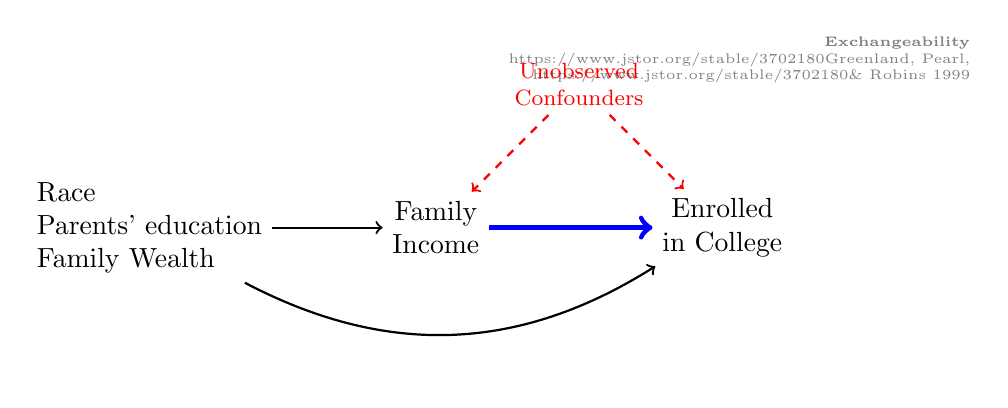
\begin{tikzpicture}[x = .3\textwidth, y = .15\textwidth]
\node at (0,1.3) {};
\node[anchor = north east, font = \tiny, gray, align = right] at (1.9,1.4) {\textbf{Exchangeability}\\\href{https://www.jstor.org/stable/3702180}{Greenland, Pearl,}\\\href{https://www.jstor.org/stable/3702180}{\& Robins 1999}};
\node at (0,-1) {};
\node[align = center] (a) at (0,0) {Family\\Income};
\node[align = center] (y) at (1,0) {Enrolled\\in College};
\node[align = left] (x) at (-1,0) {Race\\Parents' education\\Family Wealth};
\draw[->, thick] (x) -- (a);
\draw[->, thick] (x) to[bend right] (y);
\draw[->, line width = 2pt, blue] (a) -- (y);
\only<2->{
\node[align = center, red, font = \footnotesize] (u) at (.5,1) {{Unobserved}\\Confounders};
\draw[->, thick, red, dashed] (u) -- (a);
\draw[->, thick, red, dashed] (u) -- (y);
}
\end{tikzpicture}

%\onslide<3->{
%We will estimate
%\begin{itemize}
%\item how income predicts college enrollment
%\item within race, parents' education, and wealth
%\end{itemize}
%}
\end{frame}

\begin{frame}
\begin{tikzpicture}[x = \textwidth, y = .9\textheight]
\node at (0,0) {};
\node at (1,1) {};
\node[anchor = north west, align = left] at (0,1) {The \bblue{extrapolation problem}: \\
Within a population subgroup,\\
many treatments are unobserved };
\node[anchor = north east, align = right, font = \tiny, gray] at (1,1) {\textbf{Positivity}\\See \bref{https://doi.org/10.1093/aje/kwp436}{Westreich \& Cole 2011}};
\node<2->[anchor = north west] at (0,.75) {\scalebox{1.25}{\begin{tikzpicture}[x = 1in, y = 1in]
    \node[anchor = south, rotate = 90, font = \tiny, align = center] at (0,.5) {College Enrollment};
    \node[anchor = north, font = \tiny] at (.5,0) {Family Income};
    \draw[->, thick] (0,0) -- (1,0);
    \draw[->, thick] (0,0) -- (0,1);
    \draw[thick, blue] (.1,.1) -- (.5,.45);
    \draw<3>[thick, blue, dashed] (.5,.45) -- (.9,.8);
    \draw<4>[thick, blue, dashed] (.5,.45) -- (.9,.55);
    \draw[thick, gray] (.5,.8) -- (.9,.9);
    \draw<3>[thick, gray, dashed] (.1,.7) -- (.5,.8);
    \draw<4>[thick, gray, dashed] (.1,.45) -- (.5,.8);
    \node[anchor = south west, font = {\tiny\bf}, align = left] (legend)at (1.15,.7) {Population\\Subgroup};
    \draw[thick, gray] (1.1,.55) -- (1.2,.55);
    \draw[thick, blue] (1.1,.3) -- (1.2,.3);
    \node[anchor = west, font = \tiny, align = left] at (1.2,.5) {Both parents\\completed college};
    \node[anchor = west, font = \tiny, align = left] at (1.2,.2) {Neither parent\\complete\\college};
    \end{tikzpicture}
    }};
    \node<6->[anchor = north west] at (0,.2) {1) Only visualize the middle 90\% of observed treatments};
    \node<6->[anchor = north west] at (0,.12) {2) Only visualize if $n \geq 25$};
    \node<7->[anchor = north east] at (1,1) {\includegraphics[width =.3\textwidth]{figures/densities.pdf}};
\end{tikzpicture}
\end{frame}

\roadmap

\begin{frame}
How might we move on from regression?
\end{frame}

\begin{frame}
\includegraphics<1>[height = .9\textheight]{figures/stratified_0}
\includegraphics<2>[height = .9\textheight]{figures/stratified_1}
\includegraphics<3>[height = .9\textheight]{figures/stratified}
\includegraphics<4>[height = .9\textheight]{figures/stratified_gray}
\includegraphics<5>[height = .9\textheight]{figures/stratified_additive}
\end{frame}

\begin{frame}{Structure: Additive logistic regression}
\only<1>{$$\begin{aligned}
\logit\left(\frac{\P(Y = 1\mid \vec{X})}{1 - \P(Y = 1\mid \vec{X})}\right) = \alpha &+ \beta\times\log(\text{Income}) \nonumber \\
&+ \vec\gamma\times (\text{Parents' Education}) \nonumber \\
&+ \vec\eta\times (\text{Race}) \nonumber \\
&+ \vec\lambda\times \log(\text{Wealth}) \times \text{WealthTercile}
\end{aligned}$$}
\includegraphics<2>[width = \textwidth]{figures/dose_response_glm_additive}
\end{frame}

\begin{frame}{Flexibility: Generalized additive model + interactions}{\href{https://www.taylorfrancis.com/books/mono/10.1201/9781315370279/generalized-additive-models-simon-wood}{Wood 2017, R package \texttt{mgcv}}}
%Instead of $\beta\times \log(\text{Income})$, expand to a cubic spline
%\begin{itemize}
%\item TODO: EXPLAIN CUBIC SPLINE WITH FIGURE
%\end{itemize}
\begin{tikzpicture}[x = \textwidth]
\node at (0,0) {};
\node at (1,0) {};
\node<1>[anchor = west] at (0,0) {\includegraphics[width = .5\textwidth]{figures/gam_linear}};
\node<2>[anchor = west] at (0,0) {\includegraphics[width = .5\textwidth]{figures/gam_linear_points}};
\node<3>[anchor = west] at (0,0) {\includegraphics[width = .5\textwidth]{figures/gam_smooth_odds_logincome}};
\node<4>[anchor = west] at (0,0) {\includegraphics[width = .5\textwidth]{figures/gam_smooth_prob_logincome}};
\node<5->[anchor = west] at (0,0) {\includegraphics[width = .5\textwidth]{figures/gam_smooth_prob_income}};
%\node<6->[anchor = west, align = left] at (.6,0) {Smooth term for income\\$\times$ selected covariates};
\end{tikzpicture}
\end{frame}

\begin{frame}{Linear model}
\includegraphics[width = \textwidth]{figures/dose_response_gam_additive}
\end{frame}

\begin{frame}{Smooth model with interactions}
\includegraphics[width = \textwidth]{figures/dose_response_gam_educWealth}
\end{frame}

\begin{frame}{Many base learners}

\begin{itemize}
\item Standard logistic regression
\begin{itemize}
\item Additive
\item Income $\times$ Education
\item Income $\times$ Wealth
\item Income $\times$ Race
\item Income $\times$ Education $\times$ Wealth
\item Income $\times$ Education $\times$ Race
\end{itemize}
\item Each of the above, but with smooths
\end{itemize}

\end{frame}

\begin{frame}{Ensemble}
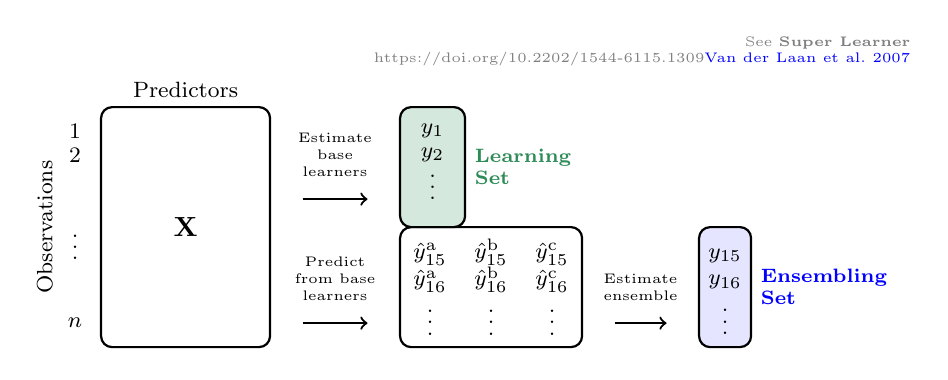
\begin{tikzpicture}[x = 6.5in, y = 4in]
\node[anchor = north east, font = \tiny, align = right, gray] at (1.2,1.1) {See \textbf{Super Learner}\\\bref{https://doi.org/10.2202/1544-6115.1309}{Van der Laan et al.~2007}};
\node[anchor = south, rotate = 90, font = \footnotesize] at (.54,.85) {Observations};
    \node[font = \footnotesize] at (.55,.97) {1};
    \node[font = \footnotesize] at (.55,.94) {2};
    \node[font = \footnotesize] at (.55,.835) {$\vdots$};
    \node[font = \footnotesize] at (.55,.73) {$n$};
    % BOX FOR X
    \draw[thick, rounded corners] (.57,1) rectangle (.7,.7);
    \node at (.635, .85) {$\mathbf{X}$};
    \node[anchor = south, font = \footnotesize] at (.635,1) {Predictors};
    \node[anchor = west, color = seagreen4, font = {\scriptsize\bf}, align = left] at (.85,.925) {Learning\\Set};
    \draw[thick, rounded corners, fill = seagreen4, fill opacity = .2] (.8,1) rectangle (.85,.85);
    \node[font = \footnotesize] at (.825,.97) {$y_1$};
    \node[font = \footnotesize] at (.825,.94) {$y_2$};
    \node[font = \footnotesize] at (.825,.91) {$\vdots$};
    \onslide<2->{
    \draw[->, thick] (.725,.885) -- node[midway, above, font = \tiny, align = center, outer sep = 5pt] {Estimate\\base\\learners} (.775,.885);
    }
    % Predict for everyone
    \onslide<3->{
    \draw[thick, rounded corners] (.8,.7) rectangle (.94,.85);
    \node[font = \footnotesize] at (.87,.77) {$\begin{matrix} \hat{y}^\text{a}_{15} & \hat{y}^\text{b}_{15} & \hat{y}^\text{c}_{15}\\\hat{y}^\text{a}_{16} & \hat{y}^\text{b}_{16} & \hat{y}^\text{c}_{16}\\\vdots & \vdots & \vdots\end{matrix}$};
    \draw[->, thick] (.725,.73) -- node[midway, above, font = \tiny, align = center, outer sep = 5pt] {Predict\\from base\\learners} (.775,.73);
    }
    % Estimate ensemble
    \onslide<4->{
    \draw[->, thick] (.965,.73) -- node[midway, above, font = \tiny, align = center, outer sep = 5pt] {Estimate\\ensemble} (1.005,.73);
    }
    \draw[thick, rounded corners, fill = blue, fill opacity = .1] (1.03,.7) rectangle (1.07,.85);
    \node[font = \footnotesize] at (1.05,.77) {$\begin{matrix} y_{15}\\y_{16}\\\vdots\end{matrix}$};
    \node[anchor = west, color = blue, font = {\scriptsize\bf}, align = left] at (1.07,.775) {Ensembling\\Set};    \end{tikzpicture} \vskip .2in
   
   % PREDICTING FROM THE ENSEMBLE
    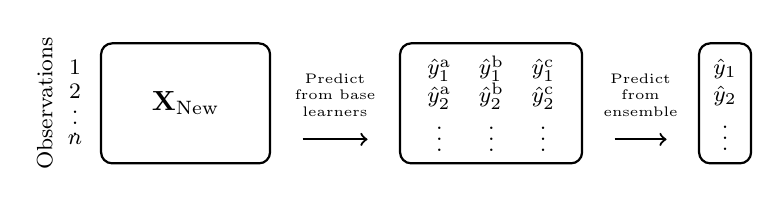
\begin{tikzpicture}[x = 6.5in, y = 4in]
    \onslide<5->{
\node[anchor = south, rotate = 90, font = \footnotesize] at (.54,.775) {Observations};
    \node[font = \footnotesize] at (.55,.82) {1};
    \node[font = \footnotesize] at (.55,.79) {2};
    \node[font = \footnotesize] at (.55,.76) {$\vdots$};
    \node[font = \footnotesize] at (.55,.73) {$n$};
    \draw[thick, rounded corners] (.57,.85) rectangle (.7,.7);
    \node at (.635, .775) {$\mathbf{X}_\text{New}$};
    }
    % Predict for everyone
    \onslide<6->{
    \draw[thick, rounded corners] (.8,.7) rectangle (.94,.85);
    \node[font = \footnotesize] at (.87,.77) {$\begin{matrix} \hat{y}^\text{a}_{1} & \hat{y}^\text{b}_{1} & \hat{y}^\text{c}_{1}\\\hat{y}^\text{a}_{2} & \hat{y}^\text{b}_{2} & \hat{y}^\text{c}_{2}\\\vdots & \vdots & \vdots\end{matrix}$};
    \draw[->, thick] (.725,.73) -- node[midway, above, font = \tiny, align = center, outer sep = 5pt] {Predict\\from base\\learners} (.775,.73);
    }
    % Estimate ensemble
    \onslide<7->{
    \draw[->, thick] (.965,.73) -- node[midway, above, font = \tiny, align = center, outer sep = 5pt] {Predict\\from\\ensemble} (1.005,.73);
    \draw[thick, rounded corners] (1.03,.7) rectangle (1.07,.85);
    \node[font = \footnotesize] at (1.05,.77) {$\begin{matrix} \hat{y}_{1}\\\hat{y}_{2}\\\vdots\end{matrix}$};
    }
    \end{tikzpicture}

\end{frame}

\begin{frame}
\includegraphics<1>[width = \textwidth]{figures/ensemble_weights}
\includegraphics<2>[width = \textwidth]{figures/ensemble_weights_positive}
\end{frame}

\begin{frame}{Ensemble results}{Estimate omitted if $n < 25$}
\includegraphics[width = \textwidth]{figures/dose_response_ensemble_educWealth};
\end{frame}

\begin{frame}{Ensemble results}{Estimate omitted if $n < 25$}
\includegraphics[width = \textwidth]{figures/dose_response_ensemble_educRace};
\end{frame}

\begin{frame}{Aggregate point estimates}
\begin{enumerate}
\item Predict at observed values
\item Predict with \$25,000 extra
\item Difference and average
\end{enumerate}
\end{frame}

\begin{frame}{Ensemble results}{Estimate omitted if $n < 25$}
\includegraphics<1>[width = \textwidth]{figures/firstdifference_ensemble_byEducWealth}
\includegraphics<2>[width = \textwidth]{figures/firstdifference_ensemble_byEducWealthRace}
\end{frame}

\begin{frame}
\huge DISCUSSION
\end{frame}

\begin{frame}

Scholars of social stratification face a tension \vskip .2in
\begin{center}
\begin{tabular}{rcl}
theory & $\rightsquigarrow$ & belief in effect heterogeneity \\
small samples & $\rightsquigarrow$ & estimation of additive models \\
\end{tabular}
\end{center} \vskip .3in \pause
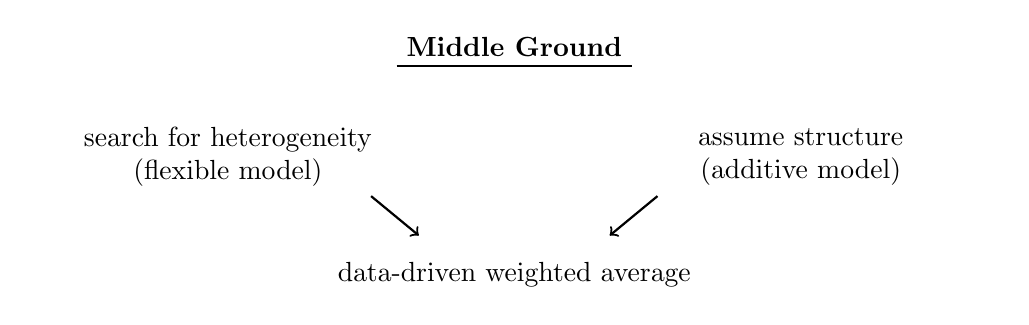
\begin{tikzpicture}[x = \textwidth]
\node at (0,0) {};
\node at (1,0) {};
\node (mg) at (.5,1.4) {\textbf{Middle Ground}};
\draw[thick] (mg.south west) -- (mg.south east); \pause
\node[align = center] at (.2,0) {search for heterogeneity\\(flexible model)}; \pause
\node[align = center] at (.8,0) {assume structure\\(additive model)}; \pause
\draw[->, thick] (.35,-.5) -- (.4,-1);
\draw[->, thick] (.65,-.5) -- (.6,-1);
\node[align = center] at (.5,-1.5) {data-driven weighted average};
\end{tikzpicture}
%\begin{itemize}
%\item Learner 1: Assume structure
%\item Learner 2: Discover heterogeneity
%\end{itemize}
%Take a data-driven weighted average
\end{frame}

\begin{frame}

\begin{tikzpicture}[x = \textwidth]
\node[anchor = west] at (0,0) {\begin{minipage}{.6\textwidth}
\bgray{Our biggest estimate:}\\
If neither parent finished college, \\
a \$25,000 income boost raises\\
college enrollment by 4 percentage points \vskip .2in \pause
\begin{itemize}
\item Take \$625,000 \pause
\item Distribute it across 25 families \pause
\item Cause 1 to enroll in college \pause
\end{itemize} \vskip .2in
The effect of family income is small
\end{minipage}};
\node<6->[anchor = east] at (1,0) {\includegraphics[width = .3\textwidth]{figures/mayer}};
\end{tikzpicture}

\end{frame}

\begin{frame}

In a world where effects are small,\\ \pause
it is all the more important to find\\
the subgroups for whom they are larger \vskip 1in \pause
Do this with trees \hfill Athey \& Imbens 2016\\\hfill Brand et al. 2021 \\ \pause
Do this with forests \hfill Wager \& Athey 2018 \\ \pause
Do this with targeted learning \hfill Van der Laan \& Rose 2018 \\

\end{frame}

\begin{frame}%{Discussion}
 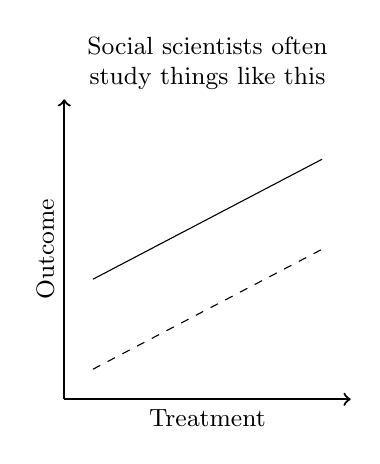
\begin{tikzpicture}[x = .3\textwidth, y = 1.5in]
    \node[anchor = south, align = center, font = \small] at (.5, 1) {Social scientists often\\study things like this};
    \draw[->, thick] (0,0) -- node[midway, below, font = \small] {Treatment} (1,0);
    \draw[->, thick] (0,0) -- node[midway, above, rotate = 90, font = \small] {Outcome} (0,1);
    \draw (.1,.4) -- (.9,.8);
    \draw[dashed] (.1,.1) -- (.9,.5);
    \end{tikzpicture} \pause
 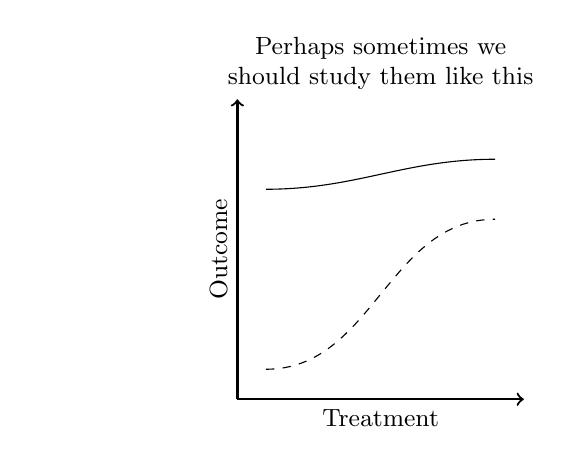
\begin{tikzpicture}[x = .3\textwidth, y = 1.5in]
    \node[anchor = south, font = \small, align = center] at (.5, 1) {Perhaps sometimes we\\should study them like this};
    \node at (-.7,0) {};
    \draw[->, thick] (0,0) -- node[midway, below, font = \small] {Treatment} (1,0);
    \draw[->, thick] (0,0) -- node[midway, above, rotate = 90, font = \small] {Outcome} (0,1);
    \draw (.1,.7) to[out = 0, in = 180] (.9,.8);
    \draw[dashed] (.1,.1) to[out = 0, in = 180] (.9,.6);
    \end{tikzpicture}
\end{frame}




\begin{frame}
\begin{center}
\large Thanks!
\end{center} \vskip .2in
\begin{small}
Ian Lundberg \hfill Jennie E. Brand \\
ilundberg@cornell.edu \hfill brand@soc.ucla.edu \\
\end{small}
\end{frame}

\begin{frame}{How did the base learners perform?}
\includegraphics<1>[height = .9\textheight]{figures/cv_0}
\includegraphics<2>[height = .9\textheight]{figures/cv}
\end{frame}

\begin{frame}{How different was machine learning?}{Effect of extra \$25k}
\includegraphics<1>[width = .7\textwidth]{figures/fd_learner_comparison_ensemble_0}
\includegraphics<2>[width = .7\textwidth]{figures/fd_learner_comparison_ensemble}
\end{frame}

\begin{frame}{Sample restrictions}

\begin{tabular}{ll}
\hline
Raw sample & 8,984 \\
Observed at age 25+ & 8,408 \\
With valid income & 6,198 \\
With income not top-coded & 6,074 \\
Non-missing wealth & 5,418 \\
Valid enrollment outcome & 4,856 \\
Valid completion outcome& 4,777 \\
\hline
\end{tabular}
\end{frame}

\begin{frame}{Standard errors}

Let $\hat\theta_1,\hat\theta_2$ be estimates that are random variables due to sampling variability. Let $\pi_1,\pi_2$ be weights on them. For simplicity, we will take the ensemble weights $\pi_1,\pi_2$ to be known, although this misses one source of uncertainty.

$$\begin{aligned}
\V(\pi_1\hat\theta_1 + \pi_2\hat\theta_2) &= \pi_1^2\V(\hat\theta_1) + \pi_2^2\V(\hat\theta_2) + 2\pi_1\pi_2\Cov(\hat\theta_1,\hat\theta_2) \\
&= \pi_1^2\V(\hat\theta_1) + \pi_2^2\V(\hat\theta_2) + 2\pi_1\pi_2\Cor(\hat\theta_1,\hat\theta_2)\text{SD}(\hat\theta_1)\text{SD}(\hat\theta_2) \\
&\leq \pi_1^2\V(\hat\theta_1) + \pi_2^2\V(\hat\theta_2) + 2\pi_1\pi_2\text{SD}(\hat\theta_1)\text{SD}(\hat\theta_2)
\end{aligned}$$

\end{frame}


\begin{frame}{First difference, by education and race}
\includegraphics[width = \textwidth]{figures/firstdifference_ensemble_byEducRace}
\end{frame}

\end{document}

